\documentclass[11pt]{letter}

%%%%%%%%%%%%%%%%%% PACKAGES %%%%%%%%%%%%%%%%%%%%%%%%%%
\usepackage[french]{babel}
\usepackage{amssymb}
\usepackage{amsmath}
\usepackage{a4wide}
\usepackage{stmaryrd}
\usepackage{amscd}
\usepackage{enumerate}
\usepackage{graphicx} %\usepackage{epsfig}
\usepackage{amsfonts}
\usepackage[utf8]{inputenc}  
\usepackage{tikz}
\usepackage{multirow}
\usepackage{array}
\usepackage{relsize}
\usepackage{listings}
\definecolor{dkgreen}{rgb}{0,0.6,0}
\definecolor{gray}{rgb}{0.5,0.5,0.5}
\definecolor{mauve}{rgb}{0.58,0,0.82}
%%%%%%%%%%%%%%%%%%%%%%%%%%%%%%%%%%%%%%%%%%%%%%%%%%
\lstset{ %
  language=python,                % the language of the code
  framerule=0pt,
  basicstyle=\relsize{-2}\ttfamily,  % the size of the fonts that are used for the code
  %backgroundcolor=\color{black!10},  % choose the background color. You must add \usepackage{color}
  showspaces=false,               % show spaces adding particular underscores
  showstringspaces=false,         % underline spaces within strings
  showtabs=false,                 % show tabs within strings adding particular underscores
  %frame=single,                   % adds a frame around the code
  rulecolor=\color{black},        % if not set, the frame-color may be changed on line-breaks within not-black text (e.g. commens (green here))
  breakatwhitespace=false,        % sets if automatic breaks should only happen at whitespace
  keywordstyle=\color{blue},      % keyword style
  commentstyle=\color{dkgreen},   % comment style
  stringstyle=\color{mauve}  
}

\begin{document}
%\pagestyle{empty}

%%%%%%%%%%%%%%%%% TITRE %%%%%%%%%%%%%%%%%%%%%%%%%%
\begin{center}
{\Large Exercices  }
\end{center}

%%%%%%%%%%%%%%%%%%%%%%%%%%%%%%%%%%%%%%%%%%%%%%%%%%%%
\textbf{Codes César}
\begin{enumerate}
   \item écrire une fonction \texttt{cesar} qui prend une clef (un nombre entre 0 et 26) et un mot (une chaîne de caractères, par exemple mot='ici')
   et qui renvoie la chaine codée. 
   \begin{lstlisting}
    def cesar(clef, mot):
         .....
         return code
   \end{lstlisting}
   Pour cela, on pourra suivre les étapes suivantes 
    \begin{itemize}
      \item créer une liste (\texttt{alpha}) qui contient l'alphabet. regarder la documentation de string.ascii\_lowercase
      \item créer la liste décalée (\texttt{decale}) de la clef (utilise une boucle, ou l'indicage des listes plus la contatenation 
      \begin{lstlisting}
        l = [1,2,3, 4]; g = l[2:] # g = [3,4]
        a = [12, 'g', -1] + ['e', '7'] #  a = [12, 'g', -1, 'e', '7']
       \end{lstlisting}
      \item créer un dictionnaire (par une boucle dic = \{\} avec pour clefs les éléments de \texttt{alpha} et pour valeurs les
      elements de \texttt{decale}
      \item avec une boucle sur la longueur de mot , crypter le mot
    \end{itemize}
   \item écrire une fonction \texttt{vraisemblance} prenant en argument un dictionnaire(une liste de chaînes de caractères), une phrase (liste
   de mots) et une clef, et qui compte le nombre de mots de la phrase decodés par la clef presents dans le dictionnaire
   \item en utilisant le squelette de programme fourni et le mini-dictionnaire, tenter de décoder la phrase suivante \\
   \begin{center}
   {\large \bf ohv pdwkv f hvw elhq} 
   \end{center} 
  

   en cherchant une clef dont la vraisemblance et superieure à 1.
\end{enumerate}

\textbf{Animation graphique}

 Le but de cet exercice est de vous montrez comment la programmation peut intervenir dans une animation graphique simple d'images de synthèse.
 On considera dans ce cadre, juste le coté géometrique de l'animation. Dans le squelette fourni en TP, on a deja un debut d'animation  : 
 une sphere qui suit une trajectoire rectiligne. 
 Pour situer la sphère aux coordonnées $(x,y,z)$ dans le repère choisi, on utilisera l'instruction \texttt{sphereActor.SetPosition(x,y,z)}
 Dans l'exemple donné on fait varier la coordonnee $z$ de la boule ce qui a pour effet de l'envoyez vers le fond de l'ecran.

 
 \begin{enumerate} 
 
    \item faire tourner le programme et essayer de programmer une trajectoire du type $y = y_0 - v_y * t$. Pour régler la position de la caméra, utiliser
    la souris et presser \texttt{e} pour lancer l'animation
    \item essayer de programmer un rebond quand on detecte des coordonnées $y$ négatives, en utilisant le schéma suivant 
   \begin{center}
     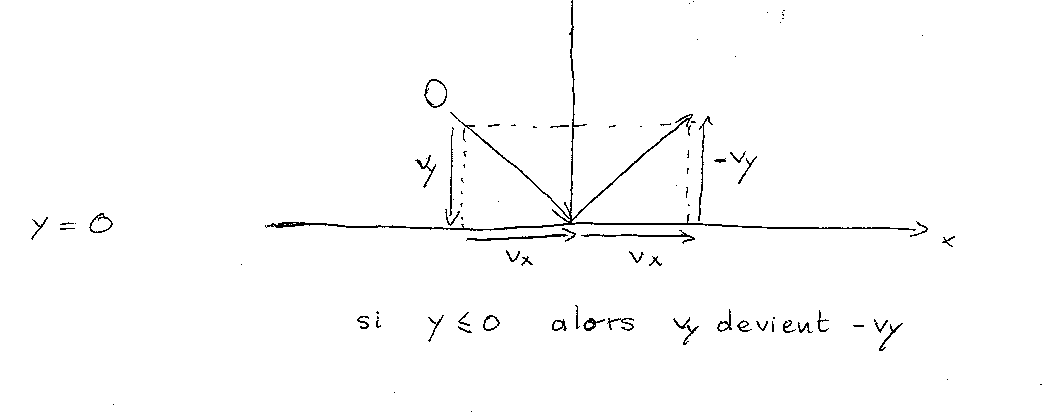
\includegraphics[width=0.8\linewidth]{rebond.pdf}
   \end{center}
   On pourra utiliser un \texttt{if} dans la boucle en temps. Bien penser à remettre $y$ à zéro pour rebondir
   \item programmer un rebond quand $y \geqslant H$
   \item on introduit de la même façon les composantes $v_x$ et $v_z$ de la vitese. Programmer les tests de bords ($x <0$, $z < 0$ et $x > L$, $z > P$)
   \item on peut ajouter du frein $vx *= -\alpha$ où $\alpha < 1$ pour ralentir la balle quand elle rebondit.
   \item voila, on a notre animation graphique!
    
  \end{enumerate}
\end{document}


